%Loosely based on "Science" journal template.

\documentclass[12pt]{article}


\usepackage{hyperref}
\usepackage{graphicx}
\usepackage{float}
\usepackage{scicite}
\usepackage{amsmath}
\usepackage{algorithmic}
\usepackage{algorithm}



% The following parameters seem to provide a reasonable page setup.

\topmargin 0.0cm
\oddsidemargin 0.2cm
\textwidth 16cm 
\textheight 21cm
\footskip 1.0cm


%The next command sets up an environment for the abstract to your paper.

\newenvironment{sciabstract}{%
\begin{quote} \bf}
{\end{quote}}


% If your reference list includes text notes as well as references,
% include the following line; otherwise, comment it out.

\renewcommand\refname{References and Notes}

% The following lines set up an environment for the last note in the
% reference list, which commonly includes acknowledgments of funding,
% help, etc.  It's intended for users of BibTeX or the {thebibliography}
% environment.  Users who are hand-coding their references at the end
% using a list environment such as {enumerate} can simply add another
% item at the end, and it will be numbered automatically.

\newcounter{lastnote}
\newenvironment{scilastnote}{%
\setcounter{lastnote}{\value{enumiv}}%
\addtocounter{lastnote}{+1}%
\begin{list}%
{\arabic{lastnote}.}
{\setlength{\leftmargin}{.22in}}
{\setlength{\labelsep}{.5em}}}
{\end{list}}



\title{Improving Immunohistochemistry Scoring Techniques for Cancer Biopsies with Computer Vision Algorithms} 



\author
{Griffin R. Calme\\
\\
\normalsize{Wayne State University}\\
\normalsize{Undergraduate Research Opportunities Program}\\
\\
\normalsize{E-mail:  griffincalme@wayne.edu}
}


\date{August 26, 2016}


%%%%%%%%%%%%%%%%% END OF PREAMBLE %%%%%%%%%%%%%%%%



\begin{document} 

% Double-space the manuscript.

\baselineskip24pt

% Make the title.

\maketitle 



% Place your abstract within the special {sciabstract} environment.

\begin{sciabstract}
  Cancers, including breast cancer, will continue to affect more lives as other modes of premature death such as infectious diseases, smoking, and accidents are declining. Immunohistochemistry offers a powerful technique for identifying proteins of interest in the tumor microenvironment. Tumor and immune proteins provide insight into the disease's characteristics and progress. Automated computer vision algorithms provide a unique ability of fast and inexpensive specimen analysis. Color deconvolution and random walker segmentation are two algorithms that, when combined in series, show consistent segmentation ability.




\end{sciabstract}

\smallskip

\indent \textit{Keywords} --- Breast cancer, color deconvolution, immunohistochemistry, random walker \indent segmentation, CD3, IL-10, IFN$\gamma$



\break
\section*{Introduction}

An estimated 12.3 percent of women in the United States will be diagnosed with breast cancer at some point in their lifetime [1]. As the number of new cases has risen over the past few decades, actual deaths from breast cancer have declined due to advances in detection and treatment. The 5-year survival rate has increased from 75.2\% in 1975 to 90.6\% in 2008 [1]. Because other causes of premature death such as infectious disease, smoking, and accidents are in decline, cancers---such as breast cancer---will continue to affect more lives. Research into the characterization of individual patient's cancers will become increasingly useful in medical practice as more people begin to live with the diagnosis and as technology advances to the point where it is feasible and clinically effective to characterize cancers based on protein expression or cellular activity in the tumor microenvironment and tailor therapy to this data.


\section*{Immunohistochemistry Theory \& Background}

Immunohistochemistry (IHC) provides a unique approach for visualizing protein expression and cell types in tumor biopsies. IHC relies on antibody-antigen reactions to tag proteins of interest for histological observation. IHC allows for the labeling of antigens \textit{in situ}, retaining morphology of the sample. As per IHC protocol, an antibody either conjugated \textit{directly} to a reporter molecule, or more usually, a secondary \textit{indirect} antibody-reporter complex is added to bind with a primary antibody---capable of binding to the target antigen [2]. The reporter molecule is usually a fluorophore or enzyme substrate. Fluorophores are a variety of chemicals capable of fluorescing in response to a defined incident wavelength of light, as used in fluorescent microscopy. Conversely, in brightfield microscopy, the enzyme substrate is usually horseradish peroxidase (HRP) or alkaline phosphatase (AP), but it can be any enzyme capable of oxidizing a chromogen [3]. The use of a primary-secondary antibody reaction is more useful than primary alone due to the signal amplification effect of multiple secondary antibodies binding to the primary [2]. Antibodies for most known antigens are widely available as are chromogens such as 3,3'-diaminobenzidine (DAB). IHC uses minimal equipment when compared with other methods of protein expression analysis [4]. 


\subsection*{IHC classification of tumor cells}

IHC stains allow for the identification of tumor cell subtypes and different lymphocytes based on surface antigens---a useful tool for characterizing cancers and the immune response [5]. IHC can be utilized in oncology to improve diagnostics, prescribing practices, and prognoses based on histological classifications of tumor subtypes [5,6]. In the treatment of breast cancer, some of the relevant therapeutic markers include estrogen receptor (ER), progesterone receptor (PR), human epidermal growth factor receptor-2 (HER-2/neu), Ki-67 and p53. Expression profiles of these proteins may classify patients into different treatment categories. Different IHC-classified subtypes of breast cancer may react differently to therapies and are correlated with different prognostic outcomes [4]. HER-2+ tumors predict positive clinical responses to Herceptin (trastuzumab), an anti-HER2 monoclonal antibody, and predicts a resistance to tamoxifen, an estrogen modulator [3-5,8]. It is becoming a more common practice to incorporate immunotherapy into the standard treatment regimen when suitable candidates are identified by IHC analysis of their tumors. 


\subsection*{IHC classification of immune cells}

In addition to characterization of the tumor by IHC, the immune response of the tumor microenvironment can also be characterized according to cellular protein expression. Lymphocyte subtypes such as CD3+, CD4+, CD8+, FOXP3+, PD1+, CTLA4+ and others can be identified based on IHC staining [2]. In addition, cytokines released into the extracellular matrix---such as interleukins, tumor necrosis factors and interferons---can be detected with IHC. This information can be factored in with tumor IHC scores to generate a broader picture of the patient's individual disease.

There is research suggesting that T cell infiltration in breast cancer is correlated with better responses to chemotherapy, increased disease-free survival (DFS), and increased breast cancer-specific survival (BCSS) [9-12]. The major subtype associated with positive clinical outcomes is CD8+ T cells. Patients with increased cytotoxic CD8+ lymphocyte tumor infiltration are more likely to have longer breast cancer-specific survival, especially in patients with triple negative breast cancers (TNBC)---negative staining for ER, PR, and HER-2/neu [9,11]. Additionally, the role of CD4+ cells in patient outcome is less clear, but the presence of this subtype does show some weak correlation with lengthened BCSS [9,10,12]. However, staining for CD4+ cells presents a problem as both T helper cells and T regulatory cells express this protein---introducing a confounding variable into the study of this relationship. This poses a significant concern as the presence of FOXP3+ T regulatory cells and PD-1+ T cells in the tumor microenvironment has been correlated with shortened DFS in certain patient groups, such as ER+ [9,10,12]. Additionally, in patients with ER+ or HER-2+ tumors, there was no CD8 to patient outcome correlation [11]. This illustrates the need for a more comprehensive understanding of relevant cells and proteins before utilizing IHC data in patient care. 


\subsection*{IHC cytokine identification}

The role of cytokine concentration in the tumor microenvironment is, likewise, unclear in regards to patient outcomes. There are many different cytokines, each with diverse physiological effects in humans. This project focuses on two of these, interleukin-10 (IL-10) and interferon gamma (IFN$\gamma$). IL-10 is known to suppress T cell activity and downregulate immune surveillance [9,13]. It has been found, counterintuitively, to provide both tumor proliferative and tumor inhibitory effects in breast cancer [13,14]. IL-10 inhibits the maturation of several antigen presenting cells (APCs) including dendritic cells. This leads to a decreased proliferation of CD4+ T cells and downregulation of T helper-associated cytokines such as IFN$\gamma$, IL-2, and tumor necrosis factor alpha (TNF-$\alpha$)[13]. Nevertheless, other results suggest that overexpression of IL-10 leads to an enhanced IFN$\gamma$ TNF, cytotoxic T lymphocyte (CTL), and natural killer (NK) cell response [14-16]. CD8+ cytotoxic T cells are known to produce IFN$\gamma$ in response to recognized tumor cells [11]. This IFN$\gamma$ is known to increase tumor permeability to granzyme B, upregulate antigen presentation, and stimulate activity of NK cells [10,17]. Various sources have been reported to show that IFN$\gamma$ is antiproliferative, antiangiogenic, and proapoptotic against tumor cells [17]. Nevertheless, other sources report finding antiapoptotic and proliferative effects of IFN$\gamma$ in certain melanomas [17]. It is unlikely that IL-10 or IFN$\gamma$ presence alone will provide reliable indicators for prognostic outcomes. Rather, once a more comprehensive picture is established of how each cytokine interacts with each cell lineage, automated image analysis of IHC-stained tumor biopsies could provide a reliable and quantitative model of the immune response to the breast tumor.


\section*{The Promises of Automation}

Historically, immunohistochemical analysis has been highly qualitative. Observers view each stained sample and search for positive staining for proteins of interest. The use of visual counting methods and qualitative scoring invariably introduces errors and biases. Human observers are prone to memory errors, produce differing counts, and require intense concentration to produce consistent results. Traditionally, histological characterization is expressed either in percentage of positively stained cells, intensity of staining or morphological characteristics of the cells. These features are used to group samples into a predefined score. There are a great deal of different grading methods in the literature and most groups use their own independent methods [18]. This problem obstructs result replication and the efforts of meta-analyses. The difference between a score of ``1+" and a score of ``2+" depends on the observer and is largely subjective---assuming the studies used numerical grades rather than highly qualitative categories such as ``intense staining" or arbitrary scales such as ``50\% staining."

The Gleason score is one popular grading system for prostate cancers. When comparing Gleason scores for different observers, it was found by R. V. Singh et al. that scores were in agreement only 43.3\% of the time, 92.3\% were within +/- 1 of agreement, with a systematic review of previous studies concluding that interobserver scoring agreement is similarly low [19]. Several other studies comparing human histological scoring found similar reproducibility issues, and have illustrated the great deal of labor and resources required for visual data gathering [20-22]. These problems stem from the fact that the human visual system is a comparative pattern analyzer rather than a quantitative system [20]. 

The time spent by human observers characterizing IHC specimens is costly and human observers scale poorly. Because two observers will not reliably give the same specimen an identical score, parallelization will yield inconsistencies. Although the human visual system is a fast pattern recognizer, iterative functions such as repeated counting are much quicker using automated computer algorithms. Additionally, the production of ordinal data (\textit{``0, 1, 2, 3"} or \textit{``none, minimal, strong"}) is much less useful for statistical analysis when compared to continuous variable data (\textit{0--100}\%) that are produced by computer programs [23]. 

Automation of this image analysis workflow using computer vision provides a good solution for the low speed, error propensity, and general heterogeneousness of human observers [18]. Nonetheless, it is imperative that human pathologists are kept as part of the IHC analysis workflow. Edge cases and complex tasks should be performed by the human pathologist, meanwhile the computer should reduce monotonous workload, and provide increased accuracy in repetitive counting tasks [18]. Applying computer algorithms to this problem promises to eliminate consistency issues as each image is put through the same program and is given a quantitative grading. Computers also have the unique property of computational speed and scalability. Computer programs can outperform human observers by several orders of magnitude in image grading speed at a fraction of the effort. Technologies such as enzyme-linked immunosorbent assay (ELISA) use similar principles to IHC. ELISA proves to be an accurate method of quantifying protein presence when used in conjunction with an automated plate reader [24]. The lack of an automated, quantitative, and standardized method for processing immunohistochemically-stained microscope slides is not a limitation of the chemistry, rather the limitation resides in current computer vision technology.


\section*{Materials}

This project used de-identified breast tumor biopsies and axillary lymph node biopsies that had been obtained from breast cancer patients at the Karmanos Cancer Institute (KCI). The biopsies were formalin fixed and embedded in paraffin blocks for sectioning with a microtome and transfer to a glass microscope slide. Specimens were de-paraffinized, stained, and fixed. CD3 was stained for with a 3,3'-diaminobenzidine (DAB) kit from GBI Labs, IL-10 and IFN$\gamma$ were stained with permanent red on two identical but separate slides using a kit from GBI Labs, and lastly hematoxylin was used as a counterstain. Primary antibodies for the CD3, IL-10 and IFN$\gamma$ were also provided by Lawrence G. Lum's BMT/Immunotherapy laboratory at KCI. A set of images was obtained by collecting both previously captured images and newly captured images, courtesy of Lawrence G. Lum's laboratory. The images were taken in brightfield at zoom levels of 4x, 10x, and 20x with digital microscopes and saved in .jpg format with low compression.


\section*{Tools Used and Project Source}

The source code and documentation are accessible through a repository on \href{https://github.com/griffincalme/MicroDeconvolution}{GitHub} (search ``MicroDeconvolution"). The \href{https://www.python.org/}{Python} programming language (version 3.5) was chosen for this project due to it being highly readable, quick to develop in, free, open source, and well-supported by a community of scientific computing packages. The third-party packages used include \href{http://www.numpy.org/}{NumPy} for efficient multidimensional array and linear algebra operations, \href{http://matplotlib.org/}{Matplotlib} for visualizations, and  \href{http://scikit-image.org/}{Scikit-Image} for image operations and several computer vision algorithm implementations.  


\section*{Open Source}

Open source software is software that is licensed so that users are free (as in \textit{libre}) to download, modify, contribute to, and redistribute the source code and compiled binaries. This quality can substantially increase adoption of a technology. Users are free to try out new open source programs at no cost where they might otherwise be discouraged to use proprietary tools by the cost of a license. Having the source code open increases transparency, security, and quality as it forces developers to produce software that is up to standards rather than hiding bugs, errors, and security issues by obfuscation of source code; any user or developer is free to request features and bug fixes or develop these oneself and contribute to the project. The use of open source software also encourages standardization of data formats, which allow easier sharing of data and replication of results. Lastly, the reductions in cost can potentially result in lower medical costs and more funds for research.


\section*{Review of Previous Methods}

The success and robustness of the human visual system at pattern recognition places a high bar for which software developers must exceed in order to produce a useful IHC image analysis system. Human observers are able to quickly identify a stained cell amongst a noisy background while simultaneously, and unconsciously, correcting for color distortions. The goal for computer algorithms is to replicate the superior pattern recognition of human vision while retaining the speed and reproducibility of an automated system.
	
The first obstacle in algorithm design for IHC analysis is that standard charge-coupled device (CCD) image sensors in typical microscope cameras store the picture information in three channels, red, green, and blue (RGB). The computer is initially na\"{i}ve to stain intensity. Initial solutions to this problem have been the use of hardware filters in the optical train of the microscope such as in Digital Image Subtraction, Blue Filter, Enhancement (DISBE)---which uses a blue filter to remove wavelengths of light [4]. Additionally, multispectral and hyperspectral CCD sensors that produce images in non-RGB formats can be used to isolate stain colors [6]. Hardware solutions like this cannot retroactively analyze images, have limited use for the wide variety of immunohistochemical stains available, and additional imaging equipment can add cost. Conversely, the use of software color unmixing allows any brightfield microscope to be used at minimal cost and retroactively for image sets gathered in the past or from different institutions. 
	
There are multiple algorithms for unmixing stain information from an RGB source image. Some are capable of separating pixels convoluted with more than one stain, others are not. Resulting stain maps can be binary (\textit{positive} or \textit{negative}), probability-based (likelihood of stain presence), or density-based (a continuous intensity variable) with a plethora of methods for estimating this output stain map [2,6]. Blind color decomposition has recently been proposed as a premier method for stain unmixing. This method models absorption, uses a standard CCD camera, produces a density map, and is able to unmix pixels with two stains present [6]. Unfortunately, a key requirement of this algorithm is that the stains used must model the Beer-Lambert Law of light absorption. 3,3'-Diaminobenzidine (DAB), one of the most common and widely-available immunohistochemical stains, produces color via scattering rather than pure absorption and thus does not follow the Beer-Lambert relationship [2,6,24,25]. Color deconvolution as developed by Ruifrok \& Johnston remains the most promising candidate for unmixing RGB information, it is capable of separating up to three stain channels into a density map using standard RGB images [6,25,26]. 

\begin{figure}[H]
  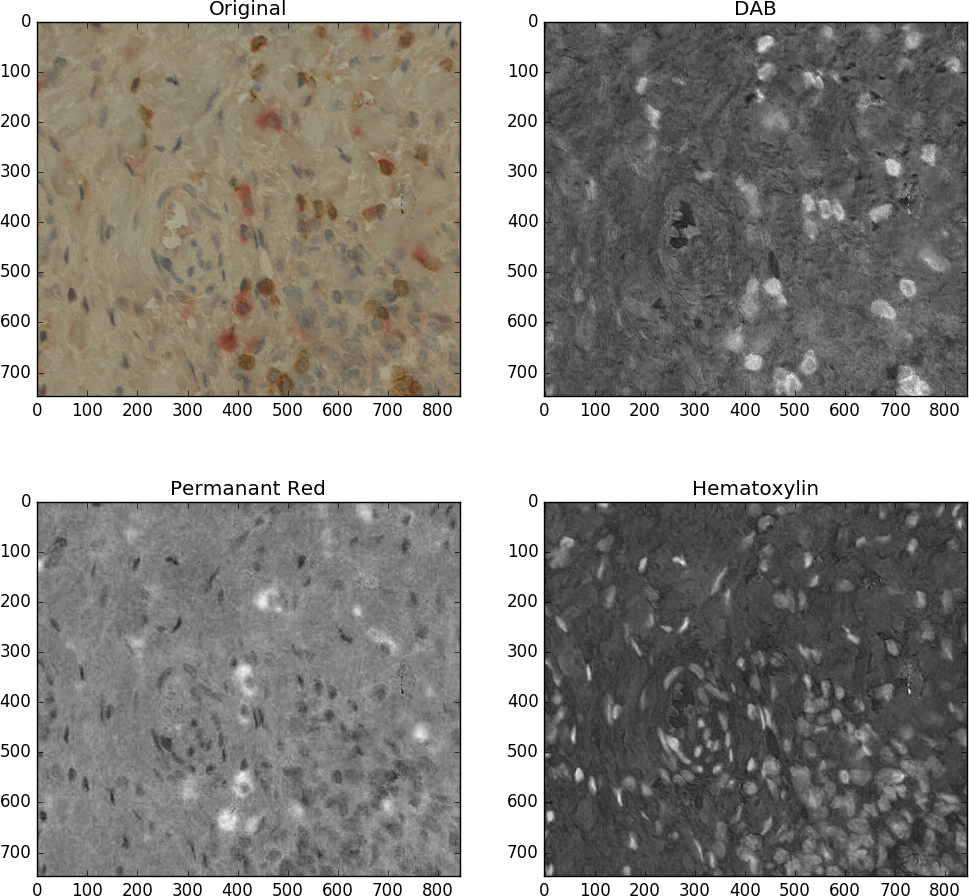
\includegraphics[width=\linewidth]{1CD.png}
  \caption{Color deconvolution for three stain channels. White signifies more intensity, black signifies less. IHC specimen stained for CD3 with DAB, Hematoxylin, and IL-10 with permanent red.}
  \label{fig:ColorDeconvolution1}
\end{figure}

\newpage

After the stain intensity map is generated for each stain, segmentation algorithms are required to quantify the resulting stain. The simplest algorithm for this is the global threshold. In this process a threshold number is pre-defined and all pixels below that value of intensity are marked as negative [2]. The pixels above that value can either be marked as positive to produce a binarized result or the intensity information can be conserved for analysis.



\begin{algorithm}
\caption{Binarized Global Threshold}
\begin{algorithmic} 
\FORALL{$pixels$}
\IF{$I < T$}
\STATE $I = 0$
\ELSIF {$I \geq T$}
\STATE $I = 1$
\ENDIF
\ENDFOR
\end{algorithmic}
\end{algorithm}

\begin{algorithm}
\caption{Global Threshold with Information Conservation}
\begin{algorithmic} 
\FORALL{$pixels$}
\IF{$I < T$}
\STATE $I = 0$
\ELSIF {$I \geq T$}
\STATE $I = I$
\ENDIF
\ENDFOR
\STATE
\STATE Where \textit{I} is the pixel's intensity
\STATE and \textit{T} is the threshold value
\end{algorithmic}
\end{algorithm}


\noindent The use of global thresholds is not suitable for majority of IHC images, which tend to have poorly defined contrast and where the edges of the image are often darker than the center due to uneven illumination [2]. Thresholds also fail to interpolate for pixels that reside interior to groups of positively identified pixels, a key goal of segmentation. Lastly, pixel-based thresholds often leave spurious false positive hits.


\begin{figure}[H]
  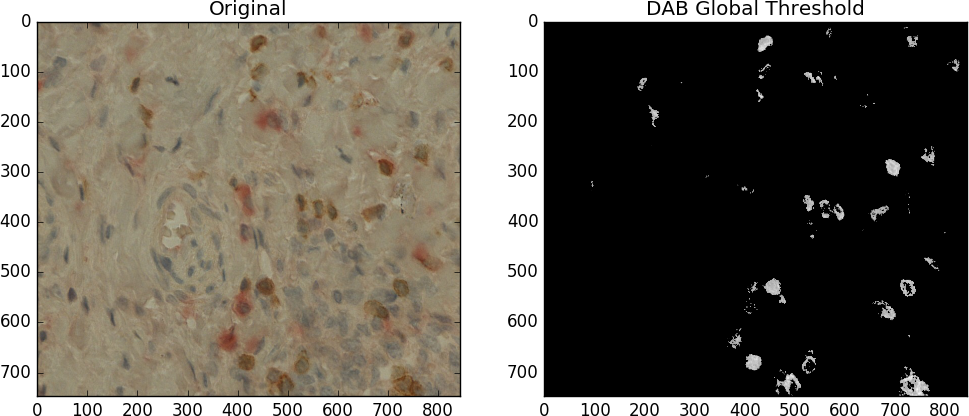
\includegraphics[width=\linewidth]{2DABglobal.png}
  \caption{Comparison of DAB global threshold with intensity conservation at T = 0.5 (50\%). IHC specimen stained for CD3 with DAB, Hematoxylin, and IL-10 with permanent red.}
  \label{fig:DABglobal2}
\end{figure}


Adaptive thresholds have the potential to correct for regional variations in lighting by utilizing localized intensity information to determine the threshold value for each pixel based on the defined regional block size [2,27]. This method, by definition, does not allow for defining a threshold intensity and so easily fails to capture what the observer is looking for in a positive-negative boundary condition. Edge-based detection using the \textit{Canny edge detector}, \textit{Sobel operator}, and other methods have also been proposed as segmentation methods. These methods are error prone due to noise, poorly defined boundaries between stain and background, and overlapping cells [2]. Pre-trained feature detectors like \textit{Haar cascades}, that identify objects based on an idealized template of features (highly effective in face detection) also fail due to large inter-cellular heterogeneity [2]. Yet, other researchers have proposed using blob-detection algorithms such as \textit{Difference-of-Gaussian} (DoG) that detect blob-like regions which stand out from the background based on intensity [28]. This method would seem promising due to the globular nature of cells, but it lacks resiliency for overlapping cells and cells of different sizes and shapes---all common occurrences in IHC specimens. In addition, blob detection fails to be useful for quantifying cytokines, which can be amorphously diffused in the extracellular matrix, as it is inherently cell-based rather than area-based segmentation.

\begin{figure}[H]
  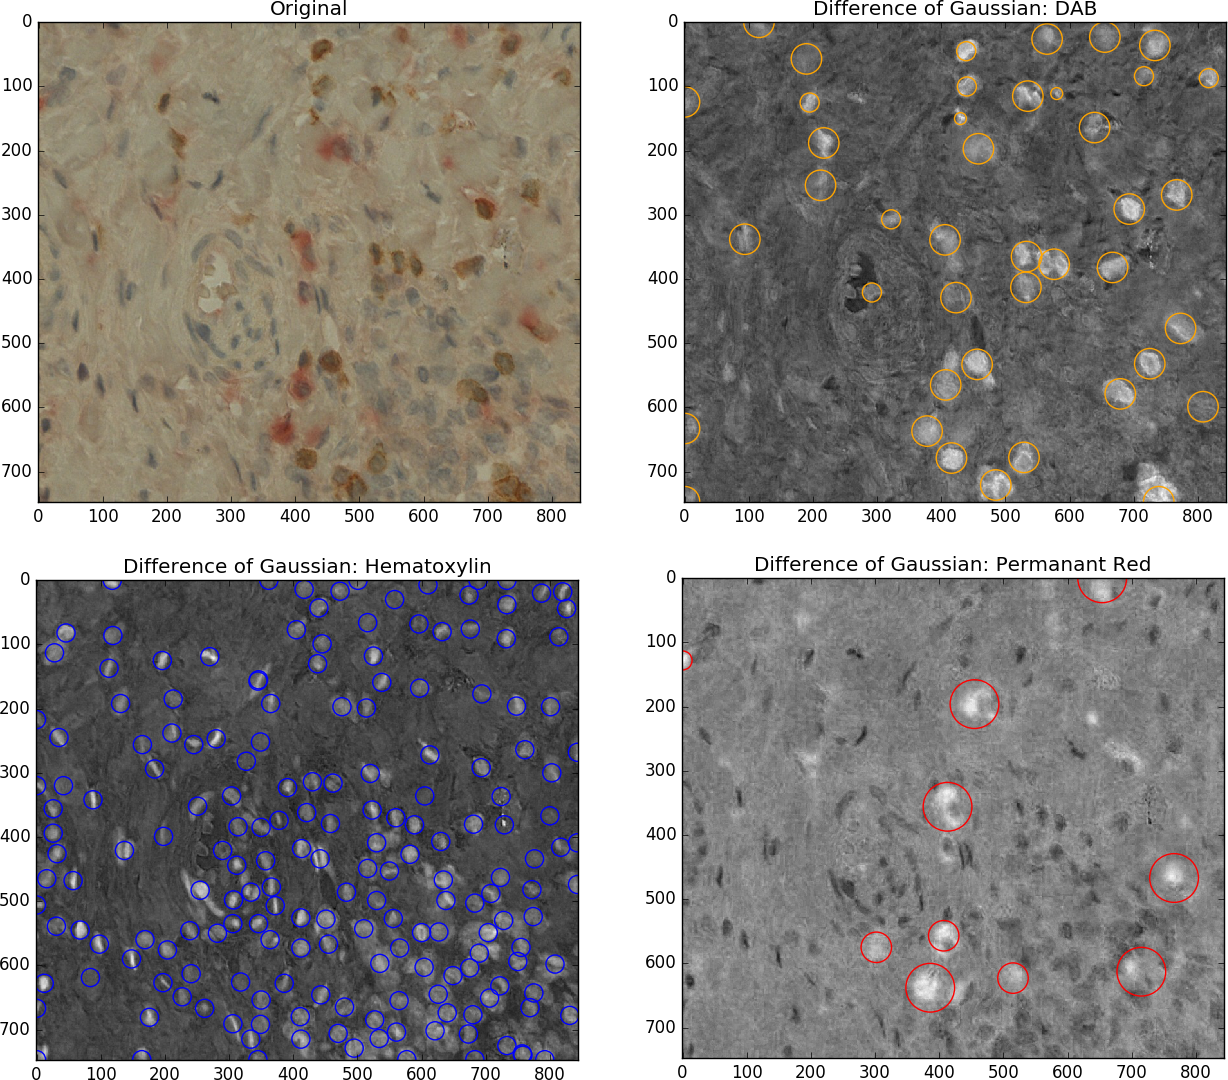
\includegraphics[width=\linewidth]{3BlobDetect.png}
  \caption{T-cell, cell nuclei, and IL-10 blob detection. Specimen stained for CD3 with DAB, IL-10 with permanent red, and a hematoxylin counterstain. N\textsubscript{DAB}= 42, N\textsubscript{hema}= 188, N\textsubscript{red}= 10.}
  \label{fig:BlobDetect3}
\end{figure}



\begin{figure}[H]
  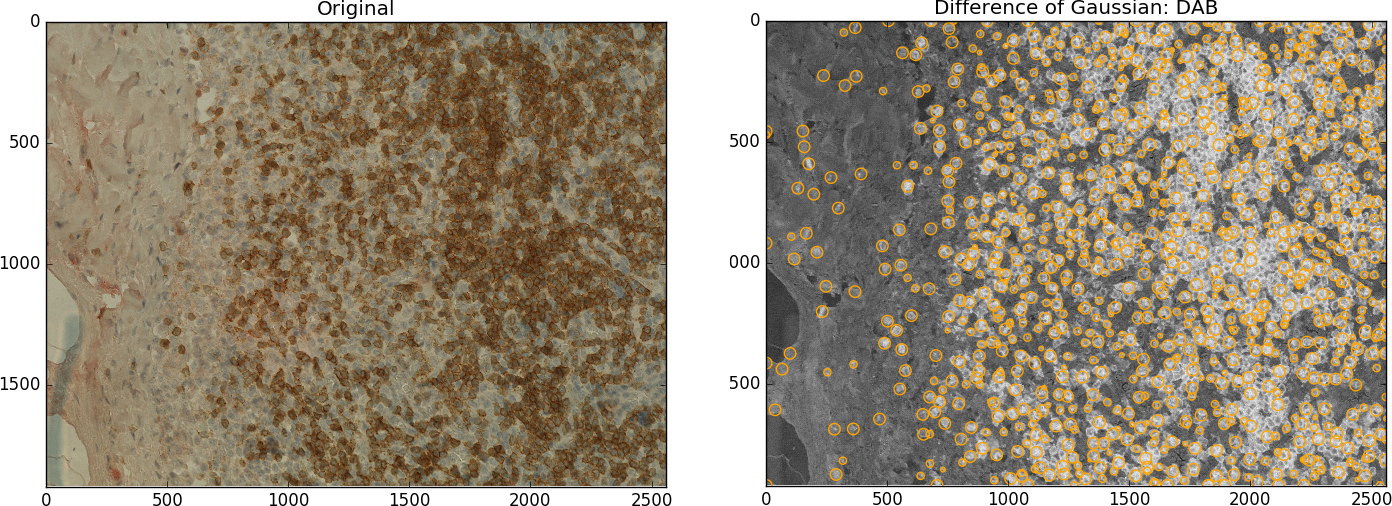
\includegraphics[width=\linewidth]{4BlobDetectHard.png}
  \caption{T-cell blob detection. IHC specimen stained for CD3 with DAB, Hematoxylin, and IL-10 with permanent red.  Example of overlapping cells causing systemic false negatives. N\textsubscript{DAB}= 918.}
  \label{fig:BlobDetectHard4}
\end{figure}


Lastly, other research has recommended seeded watershed segmentation. This method is successful with overlapping cells and can be used for both cells and diffused cytokines [2,29,30]. Watershed is much more successful at interpolating stain area, but does not easily produce uniform boundaries without further post-processing. Area-based segmentation algorithms that calculate stain coverage, contrary to human methods of segmentation, may be far more successful at quantifying staining when compared to cell-based counting [28].
	
For this project, \textit{random walker segmentation} (RWS) was used as developed by Grady (2006) [31]. It takes similar inputs and produces similar results as watershed segmentation. RWS also takes seeds and uses these to calculate object boundaries. The algorithm was originally designed to be user interactive, users could mark seeds and then use a random walker program to segment based on the seeds, however this is incredibly time consuming for large histological image sets [30,31]. The seeds can be determined algorithmically, without user input, by setting a global threshold for seed marking. It solves the problems associated with interpolation of cell area, overlapping cells, and it is resilient to noise. RWS proves to produce more uniform segmentation with clearly defined boundaries, minimal false negatives for overlapping cells, and minimal spurious positive specks when compared to thresholds, blob detection and watershed segmentation.



\begin{figure}[H]
  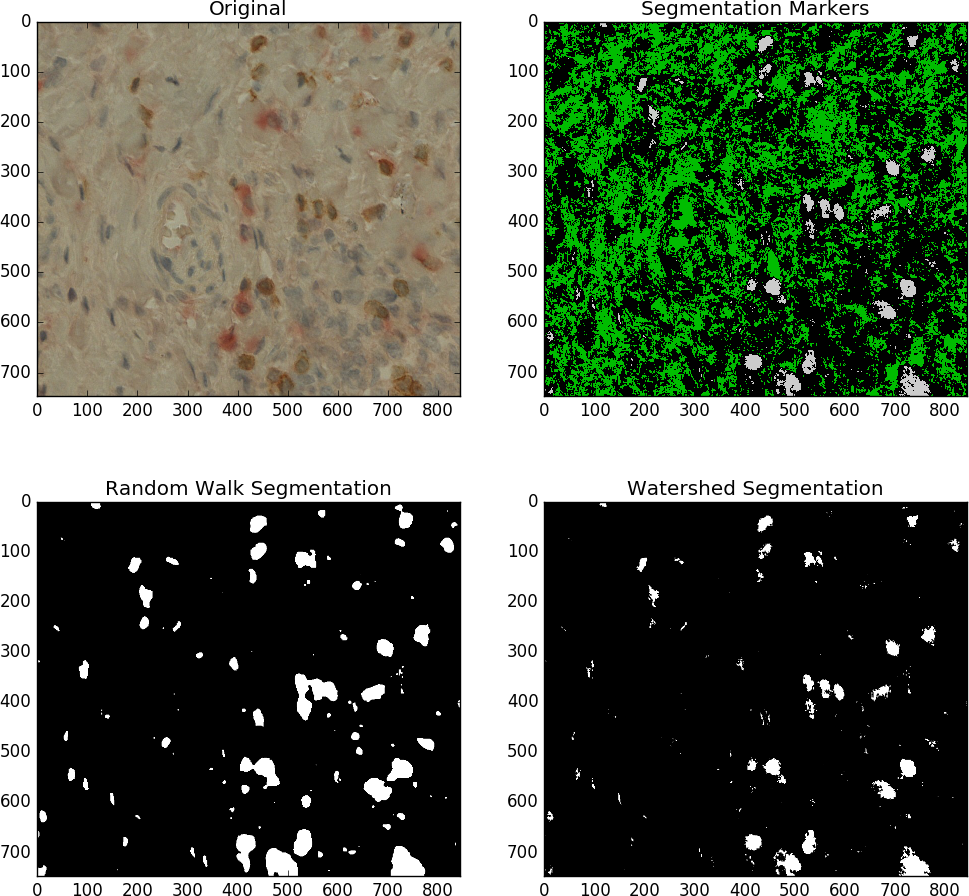
\includegraphics[width=\linewidth]{5RWSvsWatershed.png}
  \caption{DAB segmentation comparing random walker to watershed. IHC specimen stained for CD3 with DAB, Hematoxylin, and IL-10 with permanent red. Segmentation marker threshold: bottom = .3, top = .5}
  \label{fig:RWSvsWatershed5}
\end{figure}



\section*{Method \& Proposed Algorithms}
\subsection*{Flowchart Diagram}


\begin{figure}[H]
  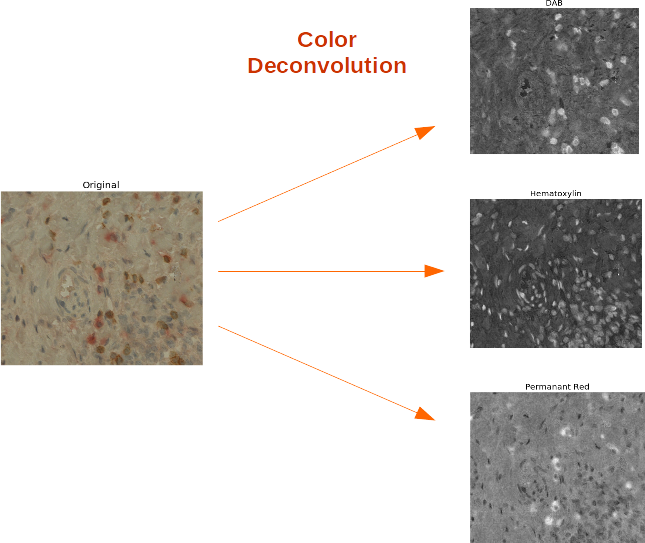
\includegraphics[width=\linewidth]{6ColorDeconvFlow.png}
  \caption{First proposed step.}
  \label{fig:ColorDeconvFlow6}
\end{figure}

\begin{figure}[H]
  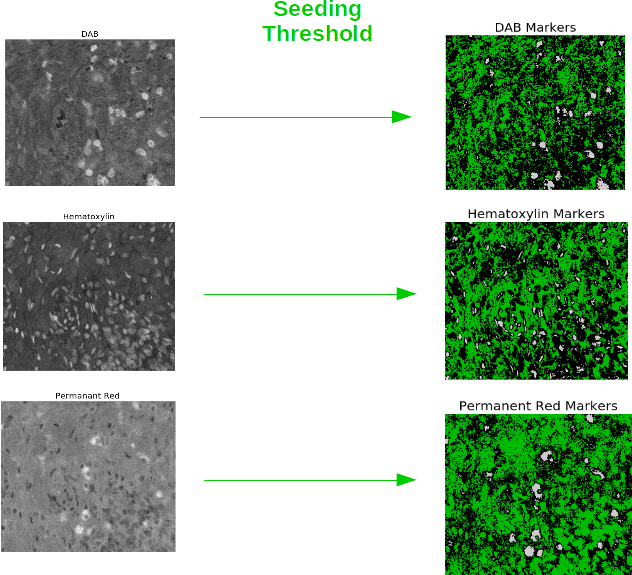
\includegraphics[width=\linewidth]{7SeedThreshold.png}
  \caption{Second proposed step.}
  \label{fig:SeedThreshold7}
\end{figure}

\begin{figure}[H]
  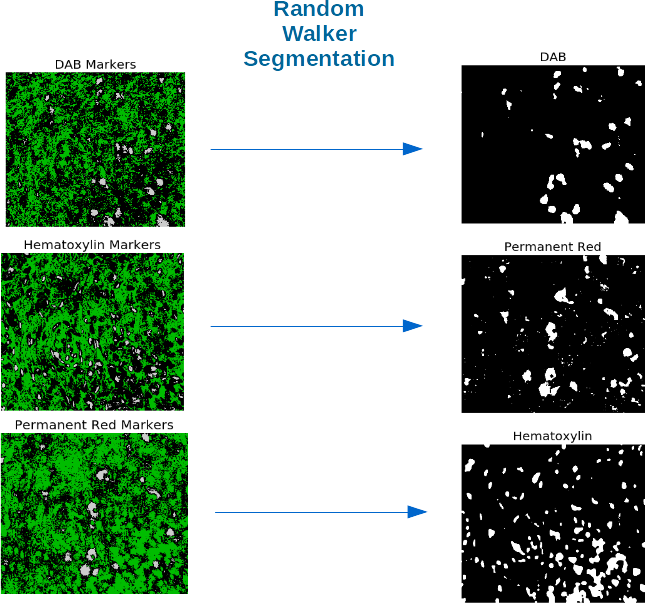
\includegraphics[width=\linewidth]{8RandomWalkSeg.png}
  \caption{Third proposed step.
  Flowchart diagram for the proposed method of IHC stain segmentation of DAB (CD3), hematoxylin, and permanent red (IL-10/IFNγ). Source image dimensions: 748x844.}
  \label{fig:RandomWalkSeg8}
\end{figure}



\begin{table}[H]
\centering
\caption{Program output}
\label{program output}
\begin{tabular}{|c|c|}
\hline
\textbf{Parameter}               & \textbf{Calculated Value} \\ \hline
DAB percent coverage             & 4.4\%                     \\ \hline
Hematoxylin percent coverage     & 11.3\%                    \\ \hline
Permanent red percent coverage   & 5.8\%                     \\ \hline
DAB \& hematoxylin area combined & 13.9\%                    \\ \hline
DAB area / (DAB \& hema)                         & 31.6\%                    \\ \hline
\end{tabular}
\end{table}


\subsection*{Color Deconvolution}

Color deconvolution (CD) is an algorithm that relies on a user-defined stain optical density (OD) matrix. It is not significantly influenced by the use of (up to) three stains, as long as they are sufficiently distinct colors [24,25]. Since the method parallels human vision in its use of RGB information, CD can separate nearly every set of three colors that can be differentiated by the human eye [25]. CD does not require special imaging equipment and functions well with a standard RGB brightfield image. For stains that follow the Beer-Lambert law, the optical density is proportional to the stain concentration [2,6,24,25], which could potentially be used to quantify protein concentration assuming the staining protocol was highly consistent across samples. This can be further complicated, however, by the fact that dyes which appear to be one color to the human observer are, in reality, composed of many different ranges of wavelengths which can overlap for two different stains [25]. Additionally, the naïve conversion of real-world full-spectrum light information into a 3 channel RGB image represents a loss of information. A potentially infinite set of wavelengths and their intensities are represented as three values (integers from 0-255, a total of 2\textsuperscript{24} colors or 24-bit color). The exact set of original wavelengths is impossible to recover and so the use of CD with RGB sensors may not be suitable for calculating stain concentration.

The Beer-Lambert Law is as defined \begin{math}I_{C} = {I_{0,C}}^{-Ac_{C}}\end{math} [25].
Where \textit{I\textsubscript{C}} is the intensity of light detected by the digital camera, \textit{I\textsubscript{0,C}} is the intensity of light transmitted through the specimen, \textit{A} is the amount of stain, and \textit{c} is the absorption factor. Lastly, subscript \textit{C} indicates the color channel. The CCD captures \textit{I\textsubscript{G}}, \textit{I\textsubscript{G}}, and \textit{I\textsubscript{B}} for each pixel of the image. The original RGB values (0-255) are as defined:



\begin{table}[H]
\centering
\caption{8 bit channel values (24-bit image)}
\label{color channel values}
\begin{tabular}{|l|l|l|l}
\cline{1-3}
R   & G   & B   &                                    \\ \hline
168 & 161 & 212 & \multicolumn{1}{l|}{Hematoxylin}   \\ \hline
236 & 32  & 80  & \multicolumn{1}{l|}{Permanent Red} \\ \hline
202 & 157 & 130 & \multicolumn{1}{l|}{DAB}           \\ \hline
\end{tabular}
\end{table}


\noindent The optical density (OD) is defined as \begin{math}OD_C = -log\textsubscript{10}\Big(\frac{I_C}{I_{0,C}}\Big) \end{math} [25]. OD\textsubscript{C} for each stain channel can be represented as a matrix of 3 (maximum) rows of a 1x3 RGB vector, one row for each stain. This matrix must be normalized with ortho-normal transformation of the RGB channels to obtain information about the effect of each stain on the overall color profile [25]. After conversion to decimal and subsequent calculation of OD, the resulting OD matrix is as follows:


\begin{table}[H]
\centering
\caption{OD Matrix}
\label{OD matrix}
\begin{tabular}{|l|l|l|l}
\cline{1-3}
R   & G   & B   &                                    \\ \hline
0.181 & 0.200 & 0.080 & \multicolumn{1}{l|}{Hematoxylin}   \\ \hline
0.034 & 0.901  & 0.503  & \multicolumn{1}{l|}{Permanent Red} \\ \hline
0.101 & 0.211 & 0.293 & \multicolumn{1}{l|}{DAB}           \\ \hline
\end{tabular}
\end{table}



\noindent The equation for normalization of the OD for each stain channel is \begin{math}\hat{p} = \frac{p_{s,c}}{\sqrt{p_{s,R}^2 + p_{s,G}^2 + p_{s,B}^2}}\end{math} [25]


\begin{table}[H]
\centering
\caption{Normalized OD Matrix}
\label{Normalized OD}
\begin{tabular}{|l|l|l|l}
\cline{1-3}
R   & G   & B   &                                    \\ \hline
0.644 & 0.710 & 0.285 & \multicolumn{1}{l|}{Hematoxylin}   \\ \hline
0.033 & 0.873  & 0.487  & \multicolumn{1}{l|}{Permanent Red} \\ \hline
0.270 & 0.562 & 0.781 & \multicolumn{1}{l|}{DAB}           \\ \hline
\end{tabular}
\end{table}

\noindent The inverse of the normalized matrix is then calculated; the result is the color deconvolution matrix. \begin{math}C = M^{-1}[y] = D[y]\end{math} [25]


\begin{table}[H]
\centering
\caption{Inverse of Normalized Matrix}
\label{Inverse Normalized}
\begin{tabular}{|l|l|l|l}
\cline{1-3}
R   & G   & B   &                                    \\ \hline
1.477 & -1.430 & 0.351 & \multicolumn{1}{l|}{Hematoxylin}   \\ \hline
0.384 & 1.540  & -1.100  & \multicolumn{1}{l|}{Permanent Red} \\ \hline
-0.787 & -0.620 & 1.950 & \multicolumn{1}{l|}{DAB}           \\ \hline
\end{tabular}
\end{table}

\noindent This final inverse matrix can be applied to the image to separate out the three stain channels.

\section*{Random Walker Segmentation}

This project used global thresholds to determine the seeds for random walker segmentation. The required seeds are then imagined to release a ``random walker" that wanders from each pixel. To simplify, the algorithm can be imagined to ask \textit{what is the probability that the individual walker will arrive at a given seed first?} The pixel is then associated with that seed for segmentation. Simulating this experiment would be computationally expensive, rather it can be done quickly by solving a system of sparse, symmetric positive-definite linear equations [31]. The random walker segmentation algorithm was originally designed to be interactive with the user. Users could mark seeds and then a program would segment images based on those seeds. The use of an intensity threshold to determine seeds utilizes the strengths of a global threshold for IHC computer segmentation, while improving results on soft boundaries and interpolation with random walker segmentation. The seeding algorithm is as follows:


\begin{algorithm}
\caption{Seeding Threshold Algorithm}
\begin{algorithmic} 
\FORALL{$pixels$}
\IF{$I < T_L$}
\STATE $S = 0$
\ELSIF {$T_U \geq I \geq T_L$}
\STATE $S = 1$
\ELSIF {$I > T_U$}
\STATE $S = 2$
\ENDIF
\ENDFOR
\STATE
\STATE Where \textit{I} is the pixel's intensity,
\STATE \textit{T\textsubscript{U}} is the upper threshold value,
\STATE \textit{T\textsubscript{L}} is the lower threshold value
\STATE and \textit{S} is the seed's type at that pixel.
\end{algorithmic}
\end{algorithm}

\newpage 

\noindent The decimal threshold values are as follows:

\begin{table}[H]
\centering
\caption{Upper \& Lower Seed Threshold}
\label{UL Seed Thresh}
\begin{tabular}{|l|l|l}
\cline{1-2}
T\textsubscript{U} & T\textsubscript{L} &                                    \\ \hline
.4   & .2   & \multicolumn{1}{l|}{Hematoxylin}   \\ \hline
.5   & .4   & \multicolumn{1}{l|}{Permanent Red} \\ \hline
.5   & .3   & \multicolumn{1}{l|}{DAB}           \\ \hline
\end{tabular}
\end{table}


\section*{Results}


\begin{figure}[H]
  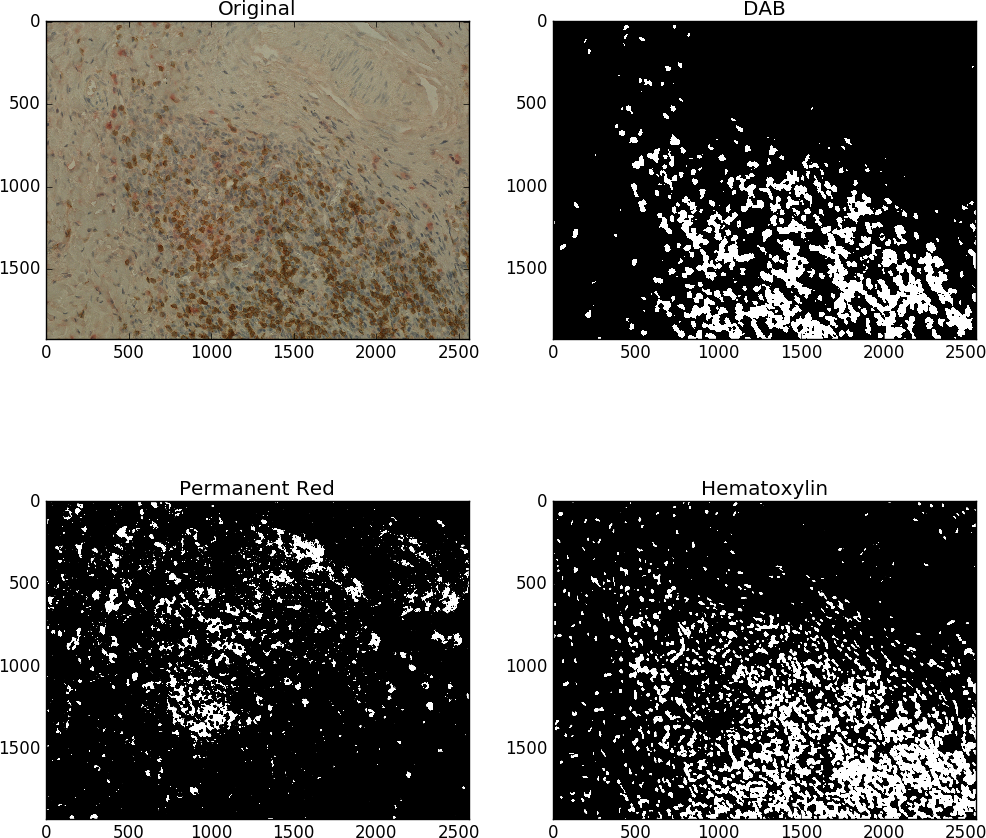
\includegraphics[width=\linewidth]{9_IL10_20x.png}
  \caption{Image dimensions 2560x1920
20x zoom, red = IL-10.}
  \label{fig:9 IL10}
\end{figure}


\begin{table}[H]
\centering
\caption{Program output}
\label{program output}
\begin{tabular}{|c|c|}
\hline
\textbf{Parameter} & \textbf{Calculated Value} \\ \hline
DAB (CD3) percent coverage & 13.8\% \\ \hline
Hematoxylin percent coverage & 18.9\% \\ \hline
Permanent red (IL-10) percent coverage & 7.4\% \\ \hline
DAB \& hematoxylin area combined & 25.1\% \\ \hline
DAB area / (DAB \& hema) & 55.0\% \\ \hline
\end{tabular}
\end{table}

%%%%%%%%%%%%%

\begin{figure}[H]
  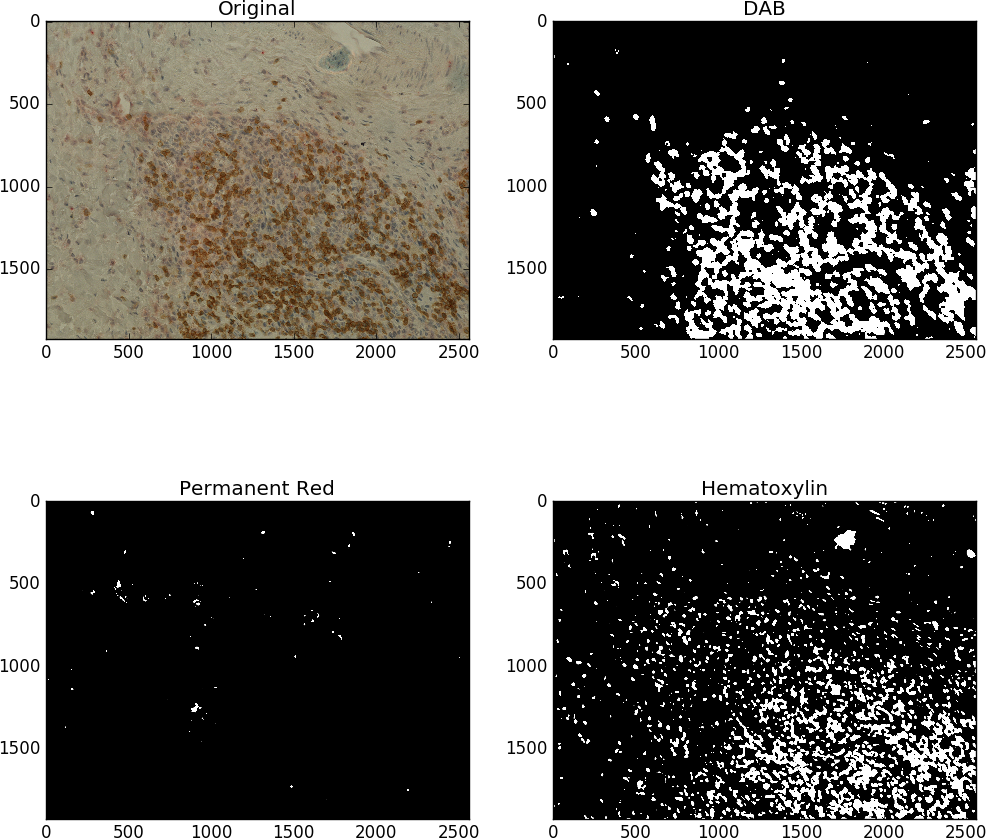
\includegraphics[width=\linewidth]{10_IFNg_20x.png}
  \caption{Image dimensions 2560x1920
20x zoom, red = IFN$\gamma$.}
  \label{fig:10 IFNg}
\end{figure}


\begin{table}[H]
\centering
\caption{Program output}
\label{program output}
\begin{tabular}{|c|c|}
\hline
\textbf{Parameter} & \textbf{Calculated Value} \\ \hline
DAB (CD3) percent coverage & 17.2\% \\ \hline
Hematoxylin percent coverage & 13.6\% \\ \hline
Permanent red (IFN$\gamma$) percent coverage & 0.2\% \\ \hline
DAB \& hematoxylin area combined & 24.7\% \\ \hline
DAB area / (DAB \& hema) & 69.7\% \\ \hline
\end{tabular}
\end{table}

%%%%%%%%%%%%%%%

\begin{figure}[H]
  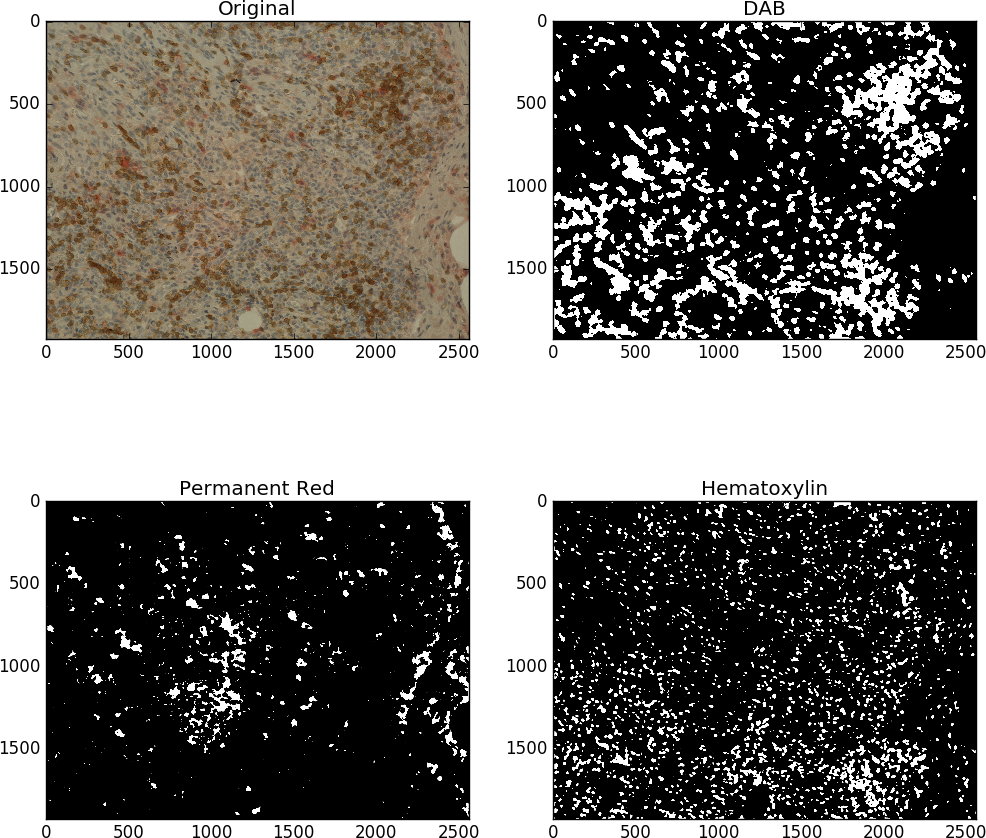
\includegraphics[width=\linewidth]{11_IL10_20x.png}
  \caption{Image dimensions 2560x1920
20x zoom, red = IL-10.}
  \label{fig:11 IL10}
\end{figure}


\begin{table}[H]
\centering
\caption{Program output}
\label{program output}
\begin{tabular}{|c|c|}
\hline
\textbf{Parameter} & \textbf{Calculated Value} \\ \hline
DAB (CD3) percent coverage & 20.3\% \\ \hline
Hematoxylin percent coverage & 10.8\% \\ \hline
Permanent red (IL-10) percent coverage & 5.1\% \\ \hline
DAB \& hematoxylin area combined & 27.9\% \\ \hline
DAB area / (DAB \& hema) & 72.9\% \\ \hline
\end{tabular}
\end{table}

%%%%%%%%%%%%%%%

\begin{figure}[H]
  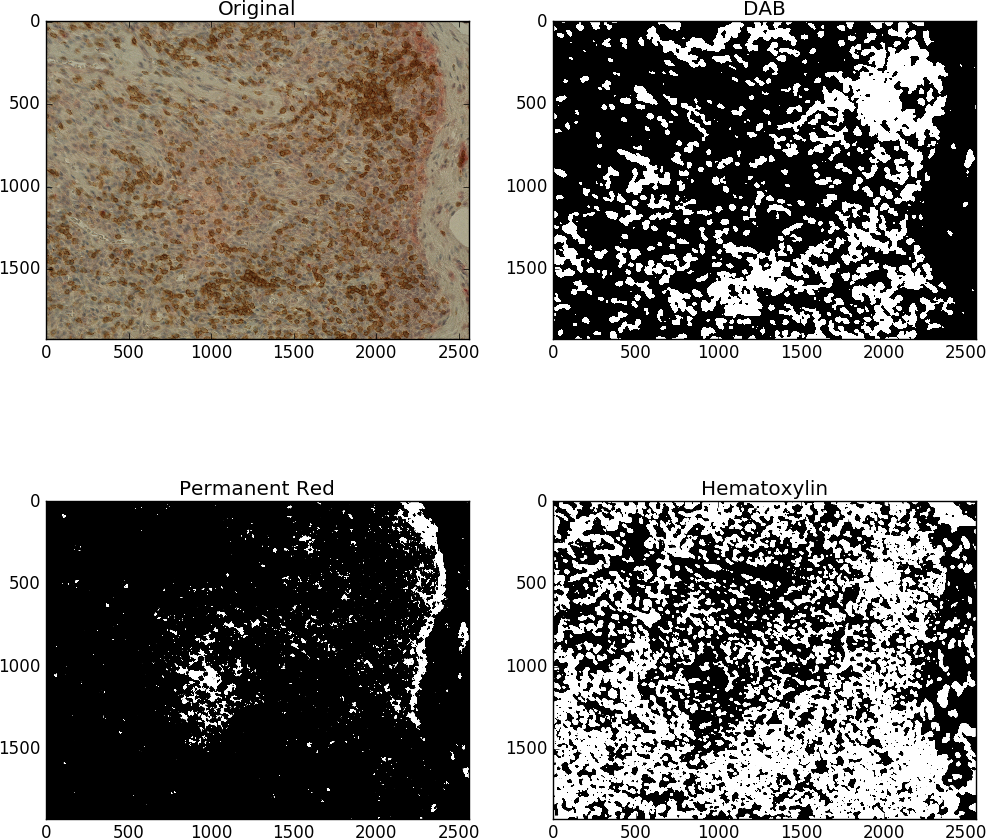
\includegraphics[width=\linewidth]{12_IFNg_20x.png}
  \caption{Image dimensions 2560x1920
20x zoom, red = IFN$\gamma$.}
  \label{fig:12 IFNg}
\end{figure}


\begin{table}[H]
\centering
\caption{Program output}
\label{program output}
\begin{tabular}{|c|c|}
\hline
\textbf{Parameter} & \textbf{Calculated Value} \\ \hline
DAB (CD3) percent coverage & 27.5\% \\ \hline
Hematoxylin percent coverage & 52.4\% \\ \hline
Permanent red (IFN$\gamma$) percent coverage & 4.6\% \\ \hline
DAB \& hematoxylin area combined & 59.8\% \\ \hline
DAB area / (DAB \& hema) & 45.9\% \\ \hline
\end{tabular}
\end{table}


\section*{Future Considerations and Discussion}

It is acknowledged that the use of staining for CD3, IL-10, and IFN$\gamma$ alone only provides
limited information of the immune response in the microenvironment. Nevertheless, the dataset
available proved to be adequate for designing the computer vision programs. Use of staining for more
specific subtypes of lymphocytes and the imaging of more types of cytokines would be of interest to
future research as there are likely to be correlations between amounts of different antigens detected and certain patient outcomes. There exists the potential to stain for many kinds of markers in the microenvironment with IHC including ER, EGFR, HER2, FOXP3, PD1, Ki-67, and any CD8+ or
CD4+ infiltration. This would give a more comprehensive picture of the activity in the
microenvironment.

Multivariate statistical models of these markers compared to patient outcomes could lead to
more accurate prognoses and more precise medicine. Automated machines could be developed for
biopsy sectioning, fixing, staining, and imaging to create highly controlled environments and obtain a
truly quantitative assessment of proteins in the microenvironment. Both color deconvolution and
random walker segmentation have linear algebra operations that could potentially be parallelized to a GPU (graphics processing unit) further increasing computational speed. Machine learning classifiers
could potentially be used to analyze this data and classify patients into diagnostic, prognostic, and
therapy categories. In this system, patients could receive care that was better tailored to their specific disease---based
on tumor markers, immune response, and cytokine profile.

The human visual system proves to be highly advanced as there are still difficulties in creating
automated computer vision systems that can replicate the resiliency of human vision to various image
imperfections. Systematic over or underestimation in automated analysis occurs due to color distortion
of images [6]. The variation of different lighting, microscopes, imaging sensors, and staining techniques create a problem for software with fixed color and threshold parameters. Hues and intensities can be shifted from the ideal that the segmentation algorithm was calibrated for. Additionally, uneven lighting, staining, and poor focus can add noise that distorts color information. In
IHC analysis, where color fidelity is of prime importance, these factors create a unique problem. While human visual systems are effective at correcting for distortions, computer algorithms must be developed to correct for these distortions in software digital image analysis.

There are a number of normalization algorithms available that can potentially solve these
problems. Some suggest normalizing stains by mapping color information of a color shifted source
image to a target image with an ideal color profile [26]. This has the potential to correct for shifted
color and intensities but introduces the possibility of erroneously shifting extreme stain profiles to the median. For example, if an image had near-complete coverage with DAB-stained cells, it would be incorrectly shifted to match the color profile of an image with average DAB staining---potentially
losing information.

A second class of color correction algorithms are the \textit{retinex} class of algorithms. These attempt to emulate the human ability of color constancy as indicated by the contraction of \textit{retina} and \textit{cortex}. Color constancy is the illusion of seeing colors in relation to their surroundings rather than by the object's color alone. The \textit{multiscale retinex with color restoration} (MSRCR) algorithm has the ability to enhance contrast locally and correct for shifted colors based on the image's background lighting, it can also be performed on the intensity channel alone to correct for brightness distortion while preserving color information [32].


\begin{figure}[H]
  \centerline{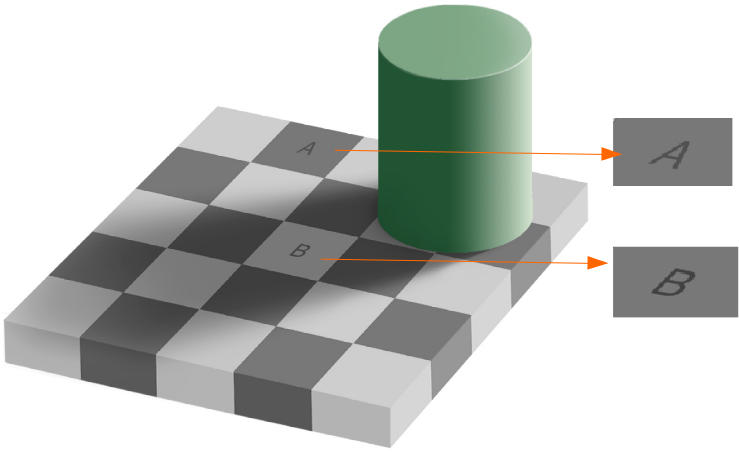
\includegraphics[width=10cm]{13ColorConstancyIllusion.png}}
  \caption{In reality, both squares A and B are the same color. In the context of the cylinder's shadow, B appears lighter than A. This is an example of the color constancy effect of human perception. [33]}
  \label{fig:Color Constancy Illusion}
\end{figure}


A final consideration is the growing field of artificial neural networks (ANN) and deep learning.
These algorithms are becoming increasingly successful at pattern recognition in both data and images
(with convolutional neural networks---CNNs). ANNs are also capable of being trained, a unique
property with great potential for the task of histological specimen analysis. Some researchers have
shown success with CNNs for cell detection, although extremely large training data sets are required if
the network is to be robust across diverse image conditions [34]. Long ANN training times also create a
problem for experimentation on novel IHC experiments, unfortunately. These two matters illustrate the
need for more open data and open software as sharing of image sets and trained classifiers would
accelerate research and the time required for these systems to reach clinical practice.

\newpage
\subsubsection*{ACKNOWLEDGMENT---The author would like to thank}

Karmanos Cancer Institute for access to digital microscopes and facilities for research. Dr. Lawrence
G. Lum for providing access to the collection of images used for this project and materials used for
staining and imaging more slides. Dr. Archana Thakur for providing guidance, visually-scored slide
data, and encouragement. Abhinav Deol for serving as the faculty mentor for the undergraduate
research project. And the Undergraduate Research Opportunities Program at Wayne State University for funding this project.


\newpage

\section*{References and Notes}

\noindent[1] SEER Stat fact Sheets: Female Breast Cancer. Surveillance, Epidemiology, and End Results
Program. http://seer.cancer.gov/statfacts/html/breast.html. Accessed August 20, 2016.

\noindent[2] Cataldo SD, Ficarra E, Macii E. Computer-aided techniques for chromogenic immunohistochemistry: Status and directions. \textit{Computers in Biology and Medicine.} 2012;42:1012-1025.

\noindent[3] Umemura S, Osamura RY. Utility of immunohistochemistry in breast cancer practice. \textit{Breast Cancer.} 2004;11:334-338.

\noindent[4] Bernardo V, Lourenço SQC, Cruz R, et al. Reproducibility of Immunostaining Quantification and Description of a New Digital Image Processing Procedure for Quantitative Evaluation of Immunohistochemistry in Pathology. \textit{Microscopy and Microanalysis.} 2009;15:353-365.

\noindent[5] Zaha DC. Significance of immunohistochemistry in breast cancer. \textit{World journal of clinical
oncology.} 2014;5:382

\noindent[6] Gavrilovic M, Azar JC, Lindblad J, et al. Blind Color Decomposition of Histological Images. \textit{IEEE
Transactions on Medical Imaging.} 2013;32:983-994.

\noindent[7] Carlson RW, Moench SJ, Hammond ME, et al. HER2 testing in breast cancer: NCCN Task Force report and recommendations. \textit{Journal of the National Comprehensive Cancer Network.} 2006; 4 Suppl 3: S1-22; quiz S23-4 [PMID: 16813731]

\noindent[8] Bilous M, Dowsett M, Hanna W, et al. Current Perspectives on HER2 Testing: A Review of National Testing Guidelines. \textit{Modern Pathology.} 2003;16:173-182.

\noindent[9] Mao Y, Qu Q, Chen X, Huang O, Wu J, Shen K. The Prognostic Value of Tumor-Infiltrating Lymphocytes in Breast Cancer: A Systematic Review and Meta-Analysis. \textit{PLoS One.} 2016;11:e0152500.

\noindent[10] Yu X, Zhang Z, Wang Z, Wu P, Qiu F, Huang J. Prognostic and predictive value of tumor- infiltrating lymphocytes in breast cancer: a systematic review and meta-analysis. \textit{Clinical and Translational Oncology.} 2016;18:497-506.

\noindent[11] Mahmoud SMA, Paish EC, Powe DG, et al. Tumor-Infiltrating CD8+ Lymphocytes Predict Clinical Outcome in Breast Cancer. \textit{Journal of Clinical Oncology.} 2011;29:1949.

\noindent[12] Gu-Trantien C, Loi S, Garaud S, et al. CD4+ follicular helper T cell infiltration predicts breast
cancer survival. \textit{The Journal of clinical investigation.} 2013;123:2873.

\noindent[13] Hamidullah, Changkija B, Konwar R. Role of interleukin-10 in breast cancer. \textit{Breast Cancer Research and Treatment.} 2012;133:11-21

\noindent[14] Mocellin S, Marincola FM, Young HA. Interleukin-10 and the immune response against cancer: a counterpoint. \textit{Journal of Leukocyte Biology.} 2005;78:1043-1051.

\noindent[15] Kundu N, Beaty TL, Jackson MJ, Amy M. Antimetastatic and antitumor activities of interleukin 10 in a murine model of breast cancer. \textit{Journal of the National Cancer Institute.} 1996;88(8).

\noindent[16] Zheng LM, Ojcius DM, Garaud F, et al. Interleukin-10 inhibits tumor metastasis through an NK cell-dependent mechanism. \textit{The Journal of experimental medicine.} 1996;184:579-584.

\noindent[17] Zaidi MR, Merlino G. The two faces of interferon-γ in cancer. \textit{Clinical cancer research: an official journal of the American Association for Cancer Research.} 2011;17:6118-6124.

\noindent[18] Cataldo SD, Ficarra E, Macii E. Computer-aided techniques for chromogenic immunohistochemistry: Status and directions. \textit{Computers in Biology and Medicine.} 2012;42:1012-
1025.

\noindent[19] Singh R, Gosavi A, Agashe S, Sulhyan K. Interobserver reproducibility of Gleason grading of prostatic adenocarcinoma among general pathologists. \textit{Indian Journal of Cancer.} 2011;48:488-495.

\noindent[20] Bernardo V, Lourenço SQC, Cruz R, et al. Reproducibility of Immunostaining Quantification and Description of a New Digital Image Processing Procedure for Quantitative Evaluation of
Immunohistochemistry in Pathology. \textit{Microscopy and Microanalysis.} 2009;15:353-365.

\noindent[21] Walker RA. Quantification of immunohistochemistry---issues concerning methods, utility and semiquantitative assessment I. \textit{Histopathology.} 2006;49:406-410.

\noindent[22] Benali A, Leefken I, Eysel UT, Weiler E. A computerized image analysis system for quantitative analysis of cells in histological brain sections. \textit{Journal of Neuroscience Methods.} 2003;125:33-43.

\noindent[23] Rizzardi AE, Johnson AT, Vogel RI, et al. Quantitative comparison of immunohistochemical staining measured by digital image analysis versus pathologist visual scoring. \textit{Diagnostic pathology.} 2012;7:42-42.

\noindent[24] Taylor CR, Levenson RM. Quantification of immunohistochemistry---issues concerning methods, utility and semiquantitative assessment II. \textit{Histopathology.} 2006;49:411-424.

\noindent[25] Ruifrok AC, Johnston DA. Quantification of histochemical staining by color deconvolution. \textit{Anal Quant Cytol Histol.} 23: 291-299, 2001.

\noindent[26] Khan AM, Rajpoot N, Treanor D, Magee D. A Nonlinear Mapping Approach to Stain Normalization in Digital Histopathology Images Using Image-Specific Color Deconvolution. \textit{IEEE Transactions on Biomedical Engineering.} 2014;61:1729-1738.

\noindent[27] Di Cataldo S, Ficarra E, Acquaviva A, Macii E. Automated segmentation of tissue images for computerized IHC analysis. \textit{Computer Methods and Programs in Biomedicine.} 2010;100:1-15.

\noindent[28] Niazi MKK, Satoskar A a., Gurcan MN. An automated method for counting cytotoxic T-cells from CD8 stained images of renal biopsies. 2013;8676:867606. doi:10.1117/12.2007977.

\noindent[29] Tuominen VJ, Ruotoistenmäki S, Viitanen A, Jumppanen M, Isola J. ImmunoRatio: a publiclyavailable web application for quantitative image analysis of estrogen receptor (ER), progesterone receptor (PR), and Ki-67. \textit{Breast cancer research : BCR.} 2010;12:R56-R56.

\noindent[30] Coelho LP, Shariff A, Murphy RF. Nuclear segmentation in microscope cell images: A hand-segmented dataset and comparison of algorithms. \textit{2009 IEEE Int Symp Biomed Imaging From Nano to Macro.} 2009:518-521. doi:10.1109/ISBI.2009.5193098.

\noindent[31] Grady L. Random Walks for Image Segmentation. \textit{IEEE Transactions on Pattern Analysis and Machine Intelligence.} 2006;28:1768-1783.

\noindent[32] Petro AB, Sbert C, Morel J. Multiscale Retinex. \textit{Image Processing On Line.} 2014;4:71-88.

\noindent[33] Grey square optical illusion. Wikimedia commons. Accessed August 25, 2016. \url{https://commons.wikimedia.org/wiki/File:Grey_square_optical_illusion.PNG}. 

\noindent[34] Chen T, Chefd'hotel C. Deep Learning Based Automatic Immune Cell Detection for Immunohistochemistry Images. In: Wu G, Zhang D, Zhou L, eds. \textit{Machine Learning in Medical Imaging: 5th International Workshop, MLMI 2014, Held in Conjunction with MICCAI 2014, Boston, MA, USA, September 14, 2014. Proceedings.} Cham: Springer International Publishing; 2014:17-24. doi:10.1007/978-3-319-10581-9\_3.


\end{document}




















